\documentclass{article}
\usepackage{graphicx}
\usepackage{amsmath}
\usepackage{amssymb}
\usepackage{mathtools}
\usepackage{amsthm}
\usepackage{geometry}
\usepackage{xcolor}
\usepackage{booktabs}
\usepackage{hyperref}
\geometry{margin=0.85in}
\setlength{\parindent}{0pt}

\newcommand{\note}[1]{\textcolor{cyan}{\textbf{**#1}}}
\newcommand{\pib}{\boldsymbol{\pi}}
\newcommand{\gb}{\boldsymbol{g}}
\newcommand{\rb}{\boldsymbol{r}}
\newcommand{\ub}{\boldsymbol{u}}
\newcommand{\vb}{\boldsymbol{v}}
\newcommand{\eb}{\boldsymbol{e}}
\newcommand{\pb}{\boldsymbol{p}}
\newcommand{\Ab}{\boldsymbol{A}}
\newcommand{\Bb}{\boldsymbol{B}}
\newcommand{\Db}{\boldsymbol{D}}
\newcommand{\Mb}{\boldsymbol{M}}
\newcommand{\Tb}{\boldsymbol{T}}
\newcommand{\Tz}[1]{\Tb^{(#1)}}
\newcommand{\Tcond}[1]{\Tb^{|#1}}
\newcommand{\one}{\boldsymbol{1}}
\newcommand{\RF}{\mathrm{RF}}
\newcommand{\omegab}{\boldsymbol{\omega}}

\title{How feature-resolved attention works, one number at a time\\
\large A pedagogical companion: from a three-state world to the use/presence split}
\author{Sprint worker B (run1\_twin)}
\date{July 15, 2026}

\begin{document}
\maketitle

This note rebuilds the theory of feature-resolved attention (FRA) from the
ground up on models small enough that every claim can be checked by hand or
by a ten-line script. Formal statements live in the companion theory note;
here every object first appears as a table of numbers from an actual run.

\section{A three-state world, in numbers}

Mess3 is a process with three hidden states and three tokens. At each step
the world moves between states and emits a token; the token both reveals
something about the current state (emission fidelity $\alpha$) and the state
drifts (transition rate $x$). For $\alpha = 0.6$, $x = 0.1$ the token-labeled
transition matrices $\Tz{z}_{ij} = \Pr(z,\, j \mid i)$ are
\begin{equation*}
\Tz{0} =
\begin{pmatrix}
0.48 & 0.02 & 0.02\\
0.06 & 0.16 & 0.02\\
0.06 & 0.02 & 0.16
\end{pmatrix},
\quad
\Tz{1} =
\begin{pmatrix}
0.16 & 0.06 & 0.02\\
0.02 & 0.48 & 0.02\\
0.02 & 0.06 & 0.16
\end{pmatrix},
\quad
\Tz{2} =
\begin{pmatrix}
0.16 & 0.02 & 0.06\\
0.02 & 0.16 & 0.06\\
0.02 & 0.02 & 0.48
\end{pmatrix}.
\end{equation*}
Token $z$ is evidence for state $z$: seeing token 0 makes state 0 likelier.
The marginal transition matrix $\Tb = \sum_z \Tz{z}$ has the uniform
stationary distribution $\pib = (\tfrac13, \tfrac13, \tfrac13)$ and
eigenvalues $\{1, \zeta, \zeta\}$ with $\zeta = 1 - 3x = 0.7$: evidence
about the state decays by a factor $0.7$ per step of world time.

An observer predicting the next token wants the \emph{belief state} (the
posterior over hidden states given tokens so far). Exact Bayesian updating
multiplies matrices --- it is inherently recursive. A single attention layer
cannot recurse; the best it can do is add up \emph{independent} contributions,
one per context position. The natural such approximation assigns each source
token a fixed displacement and decays it:
\begin{equation}\label{constrained}
\rb_d = \pib + \sum_{s=1}^{d}\, \zeta^{\,d-s}\, \gb(z_s),
\qquad
\gb(z) = \pib\,\Tcond{z} - \pib,
\end{equation}
where $\Tcond{z}$ is $\Tz{z}$ with rows normalized. Numerically the three
displacements are permutations of one vector:
\begin{equation*}
\gb(0) = (+0.141,\ -0.0705,\ -0.0705),\quad
\gb(1) = (-0.0705,\ +0.141,\ -0.0705),\quad
\gb(2) = (-0.0705,\ -0.0705,\ +0.141).
\end{equation*}
Watch both updates process the sequence $2\,2\,0\,2\,0\,1\,0\,2$:

\begin{center}
\begin{tabular}{clll}
\toprule
$d$ & token & Bayes belief & constrained $\rb_d$ \\
\midrule
1 & 2 & $(0.200, 0.200, 0.600)$ & $(0.263, 0.263, 0.474)$\\
2 & 2 & $(0.118, 0.118, 0.765)$ & $(0.213, 0.213, 0.573)$\\
3 & 0 & $(0.401, 0.134, 0.466)$ & $(0.390, 0.179, 0.431)$\\
4 & 2 & $(0.206, 0.105, 0.690)$ & $(0.303, 0.155, 0.542)$\\
5 & 0 & $(0.492, 0.116, 0.392)$ & $(0.453, 0.138, 0.409)$\\
6 & 1 & $(0.326, 0.399, 0.275)$ & $(0.347, 0.337, 0.316)$\\
7 & 0 & $(0.594, 0.229, 0.176)$ & $(0.484, 0.266, 0.251)$\\
8 & 2 & $(0.357, 0.180, 0.463)$ & $(0.368, 0.215, 0.416)$\\
\bottomrule
\end{tabular}
\end{center}

The constrained update tracks the Bayes belief but is systematically more
timid (compare $d = 2$: repeated evidence should compound multiplicatively;
a sum cannot). In cross entropy the ladder reads: Bayes $1.0809$,
constrained $1.0833$, ignore-the-context $1.0986$ nats/token --- the additive
approximation captures $86\%$ of what context is worth here.

Two remarks that will matter later. (A caution on cross entropies: the
ladder above is computed on its own evaluation set; the comparisons that
follow use a second, common evaluation set on which the same references
read Bayes $1.0790$ and constrained $1.0819$ --- CE values are only ever
comparable within one evaluation set.) First, the constrained family has an
internal \emph{gain} freedom: any probability vector minus $\pib$ lies in
the $\zeta$-eigenplane, so $\pib + \gamma \sum_s \zeta^{d-s}\gb(z_s)$ is an
equally valid ansatz for any $\gamma$. The published theory uses two
conventions that for Mess3 are parallel with $\gamma$-ratio $1.89$; the
cross-entropy-optimal gain is $\gamma^\ast \approx 1.45$ (CE $1.0802$).
Second, a trained one-layer attention-only transformer reaches CE
$1.0797$ --- better than the \emph{entire} gain family (and $0.0007$ above
Bayes on the same evaluation set). The ansatz explains
the trained model's geometry and weights, as we verify below, but the model
also exploits content-dependent pattern flexibility the ansatz does not
describe. Keeping both facts in view is the honest reading.

\section{Building the attention head by hand}

Can a softmax head produce \eqref{constrained} exactly? At first sight no:
the target weights $\zeta^{d-s}$ sum over $s$ to $(1-\zeta^d)/(1-\zeta)$,
which grows with $d$, while softmax rows always sum to $1$.

The escape uses the first position as a sink. Give every key a score that
grows linearly with its position, $\sigma(s) = s \cdot (-\ln\zeta)$, and
give position 1 alone a bonus $-\ln(1-\zeta)$. The softmax of these scores
is, exactly,
\begin{equation}\label{exactpattern}
\Ab(d, 1) = \zeta^{\,d-1}, \qquad \Ab(d, s) = (1-\zeta)\,\zeta^{\,d-s}
\ \ (s \ge 2).
\end{equation}
For $\zeta = 0.7$, row $d = 5$ reads $(0.240, 0.103, 0.147, 0.210, 0.300)$:
a clean geometric profile in the recent past, with the deficit piled onto
position 1. The row sums telescope to $1$:
$\zeta^{d-1} + (1-\zeta)(1 + \zeta + \cdots + \zeta^{d-2}) = 1$. Now let the
values carry the displacements, scaled up to undo the $(1-\zeta)$:
$f(\vb_s) = \gb(z_s)/(1-\zeta)$ for $s \ge 2$ and $f(\vb_1) = \gb(z_1)$.
Multiply pattern by values and every term is $\zeta^{d-s}\gb(z_s)$: the
constrained update, exactly, at every position. A float64 implementation
agrees with \eqref{constrained} to $3 \times 10^{-16}$.

The construction needed one luxury: position 1's value vector is smaller
than the others by exactly $(1-\zeta)$. A real transformer with additive
positional embeddings does not get that luxury --- the token part of a value
vector, $W_{OV}\,\eb(z)$, is the same at every position. With
position-independent values the best the head can do is the plain linear
score, whose softmax is the \emph{normalized} geometric profile, and the
output becomes
\begin{equation}\label{warp}
\text{output}_d = \frac{\ub_d}{1 - \zeta^{\,d}}
\qquad\text{(with } \ub_d = \textstyle\sum_s \zeta^{d-s}\gb(z_s)\text{)}:
\end{equation}
the right answer, multiplied by a position-dependent overshoot
$1/(1-\zeta^d)$ that is $3.33$ at $d{=}1$, $1.96$ at $d{=}2$, $1.32$ at
$d{=}4$, and within $3\%$ of $1$ by $d{=}10$. No choice of scores fixes
this (a constant-token sequence forces the contradiction), and no
token-independent positional value component can either, since the error is
token-dependent. We call \eqref{warp} the \emph{normalization warp}. The
trained one-layer model carries a damped version of it (measured $2.67$
against the predicted $3.33$ at $d = 1$, about $80\%$;
Figure~\ref{fig:warp}), which we propose as
the quantitative content of the previously unexplained ``first-position
scalar discrepancy'' in the constrained-belief paper --- early positions are
where softmax normalization and the target mass genuinely conflict.

\begin{figure}[t]
\centering
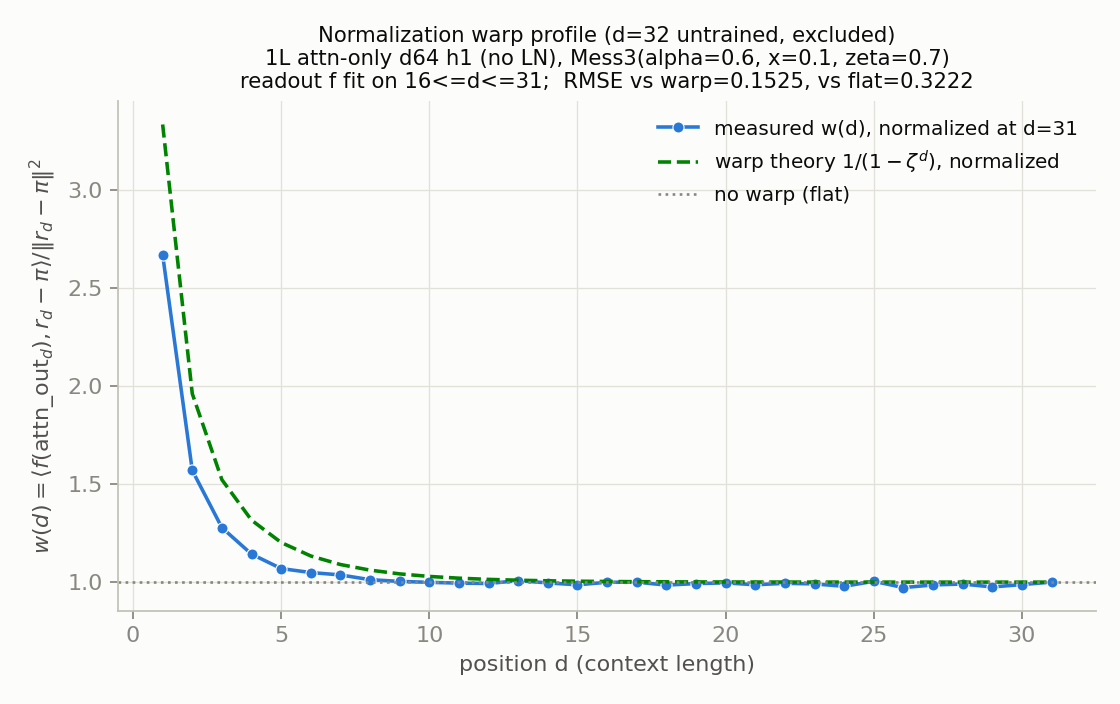
\includegraphics[width=0.62\linewidth]{../figures/phaseA_warp_profile.png}
\caption{The normalization warp in the trained one-layer model: the ratio of
the model's output magnitude to the exact constrained update, by destination
position, against the derived $1/(1-\zeta^d)$ curve and the flat (no-warp)
alternative.}
\label{fig:warp}
\end{figure}

One more question the numbers can answer: is $\zeta^k$ even the right
kernel? Freeing the lag weights $w(k)$ inside the additive family and
optimizing cross entropy directly gives a kernel with $w(0) = 1.69$
(the ansatz uses $1$) that then decays at rate $0.61$ --- faster than
$\zeta = 0.7$ --- for CE $1.08018$, beating the best gain-scaled ansatz
($1.08071$; Bayes reference $1.07959$ on this evaluation set). The
retrained positional-only transformer picks the same thing (fitted rate
$0.575$). The reason is a statistics classic: the sources are correlated
(the process mixes slowly), so optimal additive weights are
partial-regression coefficients, which shrink the redundant tail and trust
the fresh lag-$0$ evidence. And two control runs close the warp story:
kernels freed per destination row buy nothing further, and they show no
early-row boost --- the warp is the softmax's problem, not the objective's
wish.

\section{What FRA sees in QK, and why most of it is gauge}

Feature-resolved attention decomposes the score $\sigma(d,s)$ into channel
contributions: (content at $d$) $\times$ (content at $s$), content $\times$
position, and so on. Here is the trained model's score budget, as
root-mean-square score contributions over all trained $(d,s)$ pairs:

\begin{center}
\begin{tabular}{lcc}
\toprule
channel & RMS (raw) & what it decomposes into\\
\midrule
content$_q$ $\times$ position$_k$ & $2.09$ & key-position main effect $2.12$
(the lag mechanism!),\\
& & query-token main effect $0.014$ (row constant),\\
& & interaction $0.077$\\
position$_q$ $\times$ position$_k$ & $1.23$ & lag mechanism\\
content$_q$ $\times$ content$_k$ & $0.42$ & separable parts $+$
interaction $0.35$\\
position$_q$ $\times$ content$_k$ & $0.13$ & mostly common mode\\
\bottomrule
\end{tabular}
\end{center}

Read the first row twice. The biggest ``feature-involving'' channel in the
model is content-at-query $\times$ position-at-key --- and virtually all of
it is a \emph{key-position main effect}: the model reads key positions
through the shared component of the token embeddings, using content
directions as a carrier for a purely positional computation. A
feature-resolved mass accounting attributes this to ``content''; causally
it is the lag profile.

Softmax adds a second layer of emptiness: any score component constant
along a row (all $s$ at fixed $d$) cancels in the normalization. The gauge
theorem (companion note, Theorem 3.1) says that for a head whose pattern is
token-independent across sequences, \emph{every} content-involving score
term is such a row constant, one of a cancelling pair, or a positional main
effect. The one-parameter consequence checks out numerically: cutting only
token 0's key-side content perturbs the pattern by
$\mathrm{TV} = |c\varphi|\, m_d(1-m_d)$ where $\varphi$ is the common-mode
scalar and $m_d$ the attention mass row $d$ places on token-0 positions.
Measured: $\varphi = 0.323$ (constant across the row to three decimals),
and averaging $m_d(1-m_d)$ over destination rows the formula predicts a
mean TV at $c=1$ of $0.0564$ against a measured $0.0559$. (The average
must be taken per row: plugging in the mean mass $\bar m = 0.339$ would
give $0.072$ --- $m(1-m)$ is concave and the row masses vary.) The induced
loss change is predicted to five decimals.

Two honest complications, both instructive. First, the theorem's premise
holds in the trained model only \emph{on average}: flip one source token
and its attention weight moves $56\%$ relative. The model genuinely
content-gates. How much is that worth? Retrain the same architecture with
the content$\to$QK path severed (scores can only use positions) and the
loss rises from $1.07966$ to just $1.07986$: two ten-thousandths of a nat.
Cutting the same channel \emph{in place} costs $0.0034$ nats --- seventeen
times more --- because the trained model routes its positional common mode
through the content channel, and the in-place cut breaks that carrier too.
Ablation measures what the cut breaks, not what the channel is worth. The
gating also wears a disguise: its score interaction is an almost pure
same-token pattern (``attend to tokens like me'', $99.85\%$ of its
Frobenius mass, stable across four seeds), which looks like induction ---
yet adding a tunable same-token score bonus improves the loss by
$6 \times 10^{-7}$ nats (nothing), and the token-pair gate that a direct
optimizer chooses has a different, cyclic shape (cosine $0.52$ with the
learned one). SGD reliably grows an induction-\emph{looking} ornament of
essentially no causal value. And to prove the point runs in both
directions, we built a toy where induction is the \emph{task} (random
tokens with a per-sequence copy rule) and repeated the measurements: the
score interaction comes out with the same same-token shape ($99.9\%$
Frobenius share, matching Mess3's $99.85\%$) --- and there, severing it
and retraining costs $0.90$
nats where Mess3 lost $0.0002$. Same picture, four-thousand-fold
different price. Score shapes do not testify about their own importance.
Second, the basis matters: our TopK
SAE learned latents that mix token identity with position bands, and in
that basis a ``content'' cut also severs the lag mechanism (removal
fraction $0.87$ at $c=1$ versus $0.19$ for oracle content directions).
This one has a fix, and the fix teaches the right criterion. Retrain the
SAE on the residual with the per-position mean subtracted and the cut
becomes exactly oracle-like ($0.185$, at near-perfect reconstruction);
give the SAE the position index for free and it nearly does ($0.216$);
just make the dictionary $8\times$ bigger and it does not ($0.344$). And
the repaired latents still do not \emph{look} like tokens one at a time
(decoder cosine to the token embeddings $\approx 0.55$) --- TopK shreds
each token across several latents whose sum is right. What predicts cut
fidelity is whether the \emph{summed} cut contribution is a function of
token identity alone (its token-$R^2$: $1.000/0.972/0.872/0.830$, in the
same order as the damage). Judge cut sets, not latents. The
practical moral: score mass cannot tell gauge from mechanism, and an
entangled dictionary manufactures causal effects that belong to neither.

\section{What FRA sees in OV, and why it is mechanism}

The OV side transports content. At the ideal weights the attribution of the
source-$s$ token feature to the belief update at $d$ is exactly
$\zeta^{d-s}\gb(z_s)$ --- the effective-subspace-attention object of the
head-unit paper, now computed from an SAE decomposition. Severing all of it
($c=1$) should therefore delete the update entirely in one layer, and does:
three independent estimates of the severed share agree ($1.06$ from the
skip-path gauge, $1.11$ from the dose-response fit, $0.97$ from tracking),
and both use \emph{and} decodability collapse together --- a single layer
has no redundant path to preserve presence. Whatever separates use from
presence in bigger models, it is not a property of the FRA edit itself.

The multi-head caveat is sharper than we expected. On Mess3 with
$\zeta = -0.5$ the pattern must oscillate in sign, which one head cannot do:
theory forces two heads with antiparallel value circuits splitting even and
odd lags, and only their \emph{sum} is pinned to $\zeta^k$. Across five
seeds the sum indeed collapses onto one curve ($\approx 0.86\,\zeta^k$,
cosine $0.995$ with theory) --- but so do the individual heads (after
relabeling): training does not exercise its freedom; it finds the same
even/odd split every time. What does move the per-head numbers is the
\emph{training budget}: the even-lag component learns about $4\times$
slower, so head shares double between 4k and 16k steps at nearly constant
loss. If you rank heads by FRA attribution, your ranking is a function of
when you stopped training.

\section{The mixture: when the pattern goes flat}

Now change the world: draw mixing weights $\omegab$ once per sequence
(Dirichlet), then emit each token from a component chosen by $\omegab$.
The concept ``which mixture is this?'' never decays --- in spectral terms
its eigenvalue is $1$, not $\zeta$. The Bayes estimate is a count:
$\hat\omega_c(t) = (a_c + n_c)/(a_0 + t + 1)$.

What should attention do? For this \emph{exchangeable} data every lag is
equally informative, and the theory collapses to one line: the loss is a
strictly increasing function of a single scalar
$\theta = \sum_k \beta_k^2$, the inverse participation ratio of the lag
profile $\beta$ (normalized to sum to one, as softmax rows are) --- the
collision probability of two independent draws from
the profile. Spreading attention thin minimizes collisions; the flat
profile is uniquely optimal; the diagonal share drops out exactly; and no
content-gating can help. The concept is carried entirely by \emph{what} is
summed. This is the aggregation regime, now as a theorem rather than an
observation (figure \texttt{flat\_optimality.png}).

Real mixture data also has within-component grammar, whose evidence
\emph{does} decay. The optimal profile is then a superposition: a flat
floor for the concept plus a short-lag bump for the grammar. The trained
three-layer toy implements the superposition as a division of labor
(Figure~\ref{fig:twotime}): both block-0 heads are near-flat (and block-0
carries essentially all of the concept flow), both block-1 heads are
short-lag geometric, block-2 keeps one of each.

How good is the match, quantitatively? Good enough to catch a bookkeeping
error. The block-1 rates fit at $0.86$--$0.91$, which sat awkwardly above
the $0.76$ we had recorded as the grammar eigenvalue --- awkward because
the free-attention theory says optimal rates fall \emph{below} the process
eigenvalue. Computing the theory's optimal profile for the process
\emph{as actually implemented} settled it: the toy's transition matrices
carry row mass $1+x$ (so the true eigenvalue is $0.85$, not $1-3x=0.76$),
and a mixture component only advances on the steps that select it, which
slows its observable decay to $1-\bar\omega(1-\zeta) = 0.94$. The optimal
profile for that process, pushed through the same fitting script, reads
$0.87$ --- and the trained head profiles lie on the theory curve. The
lesson generalizes: before comparing a fitted rate to ``the'' eigenvalue,
make sure you know which process your data generator actually samples.

\begin{figure}[t]
\centering
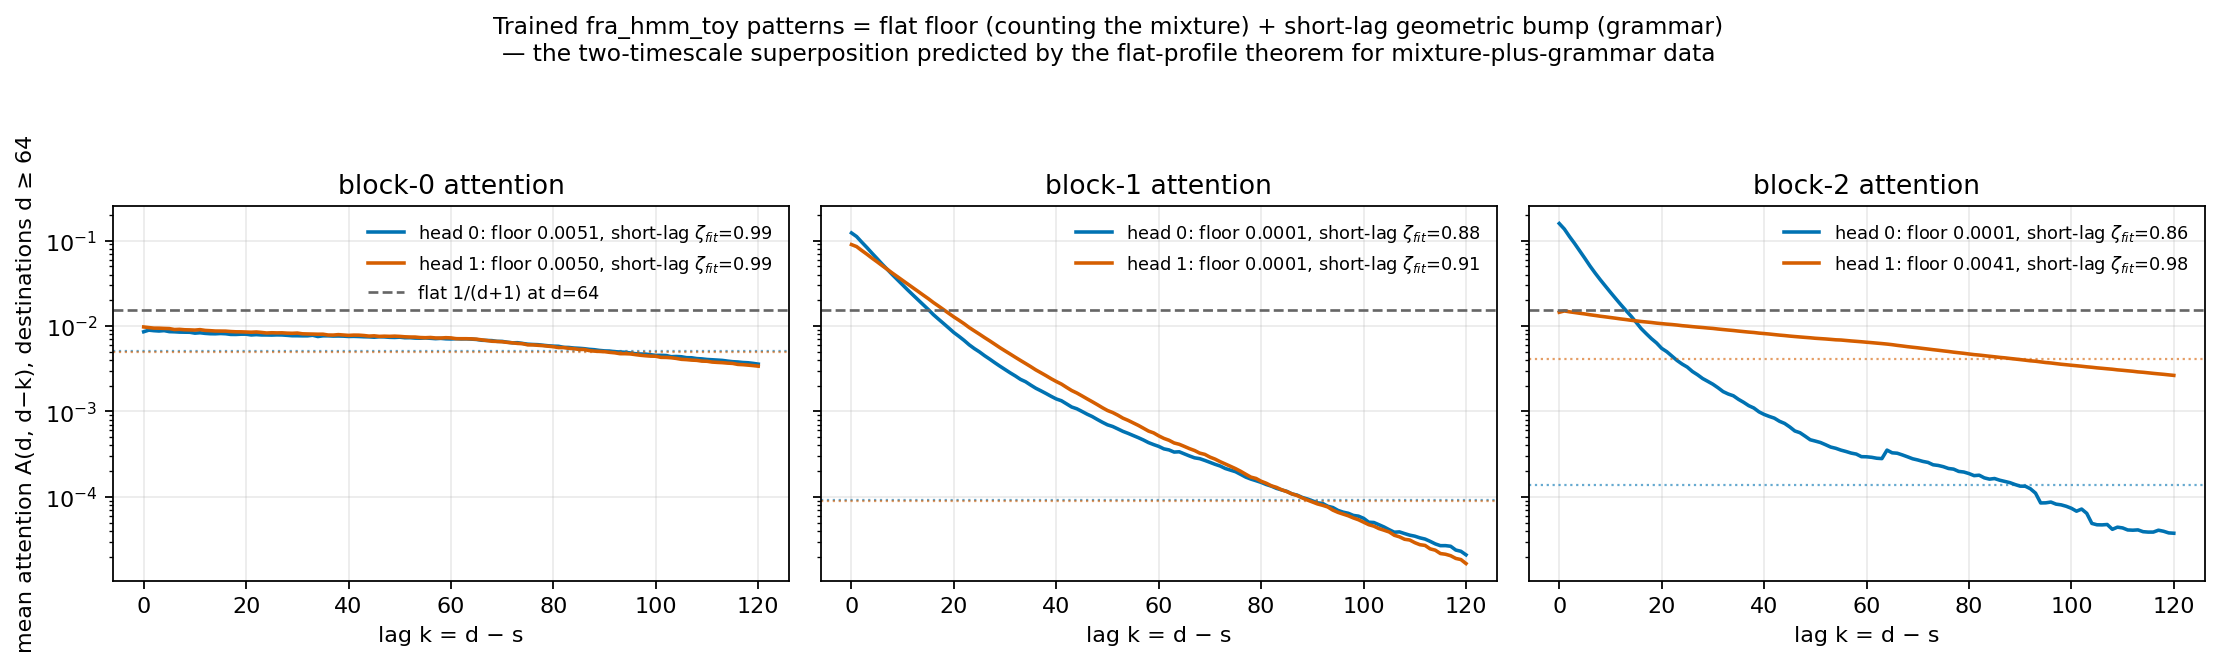
\includegraphics[width=\linewidth]{../figures/two_timescale_patterns.png}
\caption{Head specialization in the trained mixture-model toy realizes the
predicted flat-plus-geometric superposition: mean attention weight versus
lag for each head (log scale). Block-0 heads sit near the flat profile
(dashed: exactly flat attention); block-1 heads are short-lag geometric
with a negligible floor; block-2 keeps one head of each kind.}
\label{fig:twotime}
\end{figure}

\section{The intervention calculus}

In the aggregation regime many paths estimate the same count: the direct
stream carries raw tags, each attention layer re-aggregates them, deeper
layers aggregate the aggregates. Cut one path carrying a share $\rho$ of
the concept, with gain $c$, and the model's operational estimate scales by
$\kappa = 1 - c\rho$. Two laws follow, one robust and one conditional.

\textbf{The tracking null (robust).} The concept-tracking slope declines
linearly and crosses zero at $c^\ast = 1/\rho$. In a two-layer counting
transformer where the path decomposition is exact, we computed each path's
share from a clean forward pass, wrote the predictions in the results file,
then ran the sweep: predicted nulls $12.41$ and $1.94$ for two different
cuts, measured $12.405$ and $1.938$ in logit space (exactly linear,
$R^2 = 1.000$), $10.8$ and $2.17$ after the softmax. The counting model
also corrected a guess we liked: with flat heads the two layers re-estimate
the count \emph{in parallel} from raw tags ($44\%$ and $47\%$ of the
concept); the composed layer-1-into-layer-2 path carries only $8\%$.
Aggregation redundancy is parallel shallow paths, not deep composition.

\textbf{The quadratic removal law (conditional).} Near a Bayes-optimal
model the loss is \emph{stationary} in the concept signal --- the
first-order term is zero --- so the removal fraction is quadratic:
$\RF(c) \approx (c\rho)^2$. This single parabola, with one fitted
$\rho = 0.242$, reproduces the entire fra\_hmm\_toy dose-response
(Figure~\ref{fig:crho}): the null at $4.13$ versus measured
$4.0$; honest severing at $c=1$ removing $\rho^2 \approx 6\%$ --- the
famous inertness of exact severing is just the tangent parabola at the
optimum; and a parameter-free identity, removal $+$ tracking $=$ clean
tracking, flat in $c$ to $\pm 0.01$ up to the null (past it, at $c=6$, the
linear-cancellation picture drifts by $0.17$), which further reveals the cut to be a
pure contraction of the model's estimate (it scales the model's noise along
with the signal, because it is proportional to the model's own latent
activations).

\begin{figure}[t]
\centering
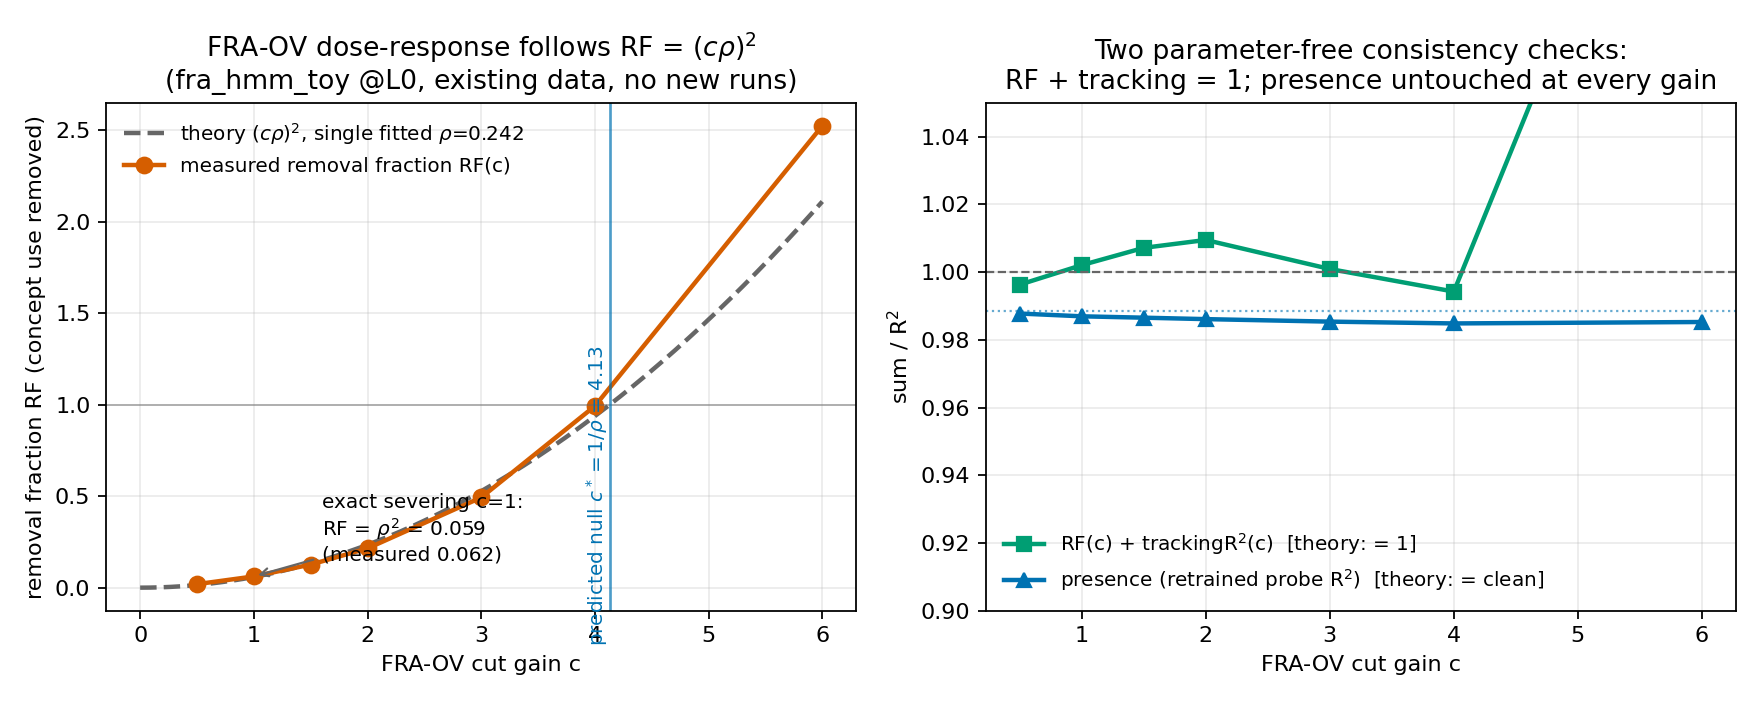
\includegraphics[width=\linewidth]{../figures/crho_law.png}
\caption{The quadratic removal law on the existing fra\_hmm\_toy gain sweep.
Left: measured removal fraction versus cut gain $c$, against $(c\rho)^2$
with the single fitted $\rho = 0.242$; exact severing ($c{=}1$) removes only
$\rho^2 \approx 6\%$, and the null lands at $c^* = 1/\rho$. Right: the
parameter-free identity $\mathrm{RF} + \mathrm{tracking} = \mathrm{const}$
holds to $\pm 0.01$ up to the null, while presence (retrained-probe $R^2$)
never moves.}
\label{fig:crho}
\end{figure}

The condition: the severed content must be a near-pure image
of the concept. fra\_hmm\_toy's cuts sever concept-selected latents ($87\%$
aligned) and obey the law; severing a whole path in the counting model
(paths are only $\sim 30\%$ concept) still costs quadratically but with a
coefficient $\gg \rho^2$, and no gain restores prior-level loss. Where
purity holds, one measurement calibrates the null:
$c^\ast = 1/\sqrt{\RF(1)} = 4.03$ against the measured $4.0$.

\section{Use versus presence}

Why does the $c^\ast$ edit null the behavior while a freshly retrained
probe still reads the concept at $R^2 = 0.985$? Count dimensions. Behavior
reads a low-dimensional projection of the residual stream; presence is the
full concept-to-residual Jacobian. A single gain is one degree of freedom:
it can zero the projection --- and only succeeds because all aggregation
paths carry \emph{proportional} copies of the same estimate, so one scalar
cancels all components simultaneously (verified: all three mixture
components hit the prior together). Zeroing the full Jacobian would need
the severed edge to be a rank bottleneck; with parallel redundant paths no
gain achieves it, so presence survives every gain, seed, and prior shift
we measured ($0.97$--$0.996$).

The counting model staged the exception that proves the rule
(Figure~\ref{fig:presence}): presence
stayed at clean levels for every gain \emph{except} exactly $c = 1$ on the
total-path cut, where it dipped to $0.755$ --- exact severing genuinely
deletes that path's copy, leaving only the parallel floor; at any other
gain the injected counter-signal is itself a decodable image of the
concept. Severing deletes; gain-tuning relocates.

\begin{figure}[t]
\centering
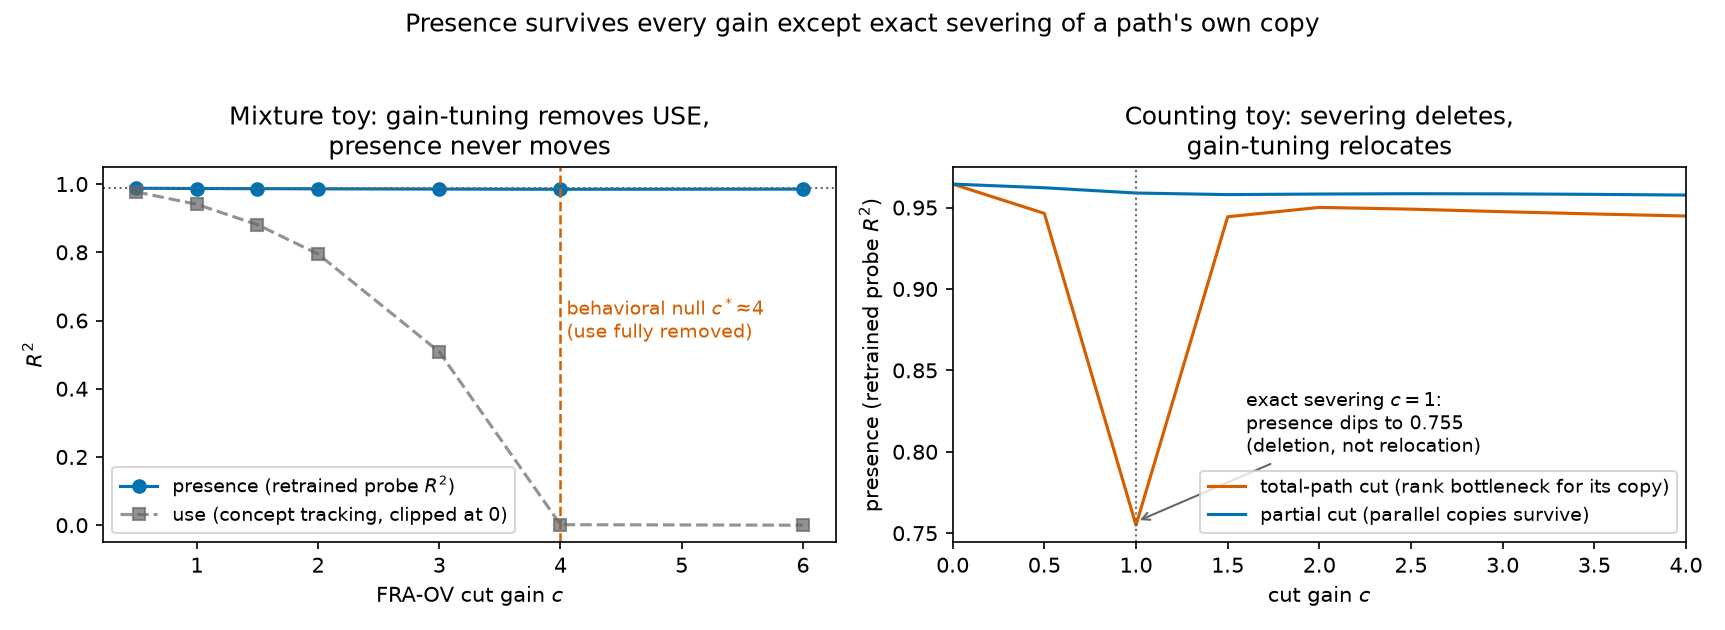
\includegraphics[width=\linewidth]{../figures/presence_vs_gain.png}
\caption{Use and presence under FRA-OV gain cuts. Left: in the mixture toy
the concept's use (tracking) declines to zero at the gain-tuned null while
its presence (retrained-probe $R^2$) never moves. Right: in the counting
toy, presence is flat at every gain except exactly $c = 1$ on the
total-path cut, where the severed path's own copy is genuinely deleted.}
\label{fig:presence}
\end{figure}

Deleting presence therefore requires cutting content at the source all
paths share --- and there the world presents its bill: the concept (the
count of block tags) and the grammar (which needs the tags) share
sufficient statistics. An observer with zero concept information pays at
least $20.8\%$ of the grammar range in collateral, for any method. ``Remove
the concept'' is two tasks --- remove its use (cheap, fragile, gain-tuned)
and remove its presence (source cuts only, taxed) --- and the toy's whole
intervention table is this section in numbers.

\section{Summary table}

\begin{center}
\small
\begin{tabular}{lll}
\toprule
FRA object & closed form at ideal weights & status\\
\midrule
QK score mass & row constants $+$ common-mode carrier & gauge (thm), causal
tests only\\
QK partial cut & $\mathrm{TV} = |c\varphi| m(1-m)$ & verified to 4 decimals\\
OV attribution & $\zeta^{d-s}\gb(z)/(1-\zeta^d)$ & verified; per-head =
checkpoint-dependent\\
\midrule
intervention & law & domain\\
\midrule
OV cut, tracking & slope $1 - c\rho$, null $c^\ast = 1/\rho$ & robust
(exact in logits)\\
OV cut, loss & $\RF = (c\rho)^2$, $c^\ast = 1/\sqrt{\RF(1)}$ & concept-pure
cuts\\
QK cut & inert: gauge $+$ counting robustness & aggregation regime\\
source content cut & only presence reducer & pays entanglement tax\\
\midrule
basis diagnostic & criterion & fix\\
\midrule
cut-set fidelity & token-$R^2$ of the \emph{summed} cut feature &
position-demeaned SAE inputs\\
\bottomrule
\end{tabular}
\end{center}

\end{document}
